\chapter{実験結果}\label{RS}


%----------7.1--------
\section{アンケート結果}


\begin{figure}[tb]
	\begin{center}
		\includegraphics[scale=0.5]{img/diffidence.eps}
		\caption{協調プログラミングにおけるフォロワの遠慮}
		\label{fig:Diffidence}
	\end{center}
\end{figure}

%\samepage

\begin{figure}[tb]
	\begin{center}
		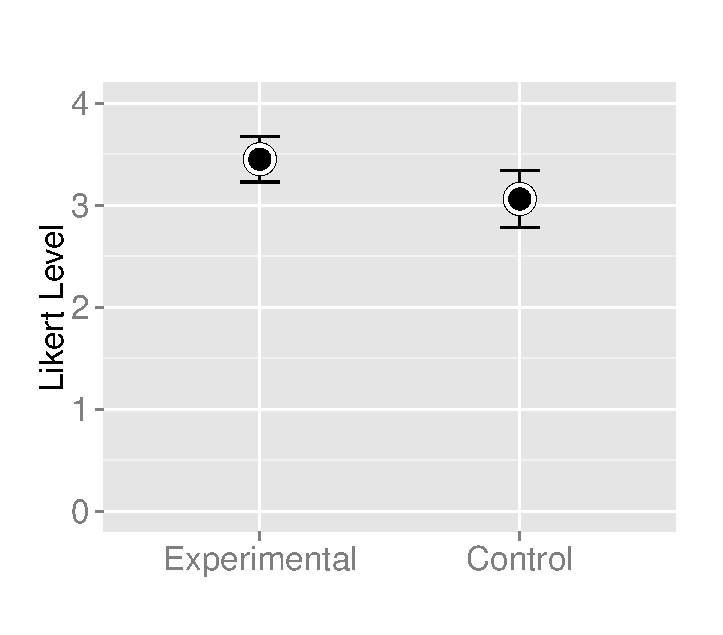
\includegraphics[scale=0.5]{img/contribution.eps}
		\caption{協調プログラミングにおけるフォロワの貢献}
		\label{fig:Contribution}
	\end{center}
\end{figure}


フォロワのアンケートの有効回答数は,53件(利用群20件,非利用群33件)であった.

「グループでプログラムを組むときに他のメンバーに対して遠慮しましたか」と尋ねたアンケートの結果を\figref{fig:Diffidence}に示す.図のエラーバーは95\%信頼区間を表す.利用群の平均は3.05(sd=0.80),非利用群の平均は2.55(sd=0.89)であった.t検定を行った結果,利用群と非利用群の平均の差は有意であった(両側検定:t(43.1)=2.08,p$<$.05).


「あなたはあなたのグループの作品作りに貢献できましたか」と尋ねたアンケートの結果を\figref{fig:Contribution}に示す.図のエラーバーは95\%信頼区間を表す.利用群の平均は3.45(sd=0.49),非利用群の平均は3.06(sd=0.81)であった.t検定を行った結果,利用群と非利用群の平均の差は有意であった(両側検定:t(50.1)=2.12,p$<$.05).


\begin{table}[tb] 
\caption{グループでのプログラミングの感想} 
\label{tab:free1}
\hbox to\hsize{\hfil
\begin{tabular}{c|p{7cm}}\hline\hline
S01	& いろんなアイディアが出てくるので、個人で作るよりも楽しく取り組めました。また、自分が分からないことを他のメンバの子が教えてくれたりしたのでよかったです。 \\\hline
S02	& 「○○をやりたい」という目的が同じでも、人によってやり方が違うのが面白いなと思った。\\\hline
S03	& グループ内での実力さが大きく、自分にできることを探すのに苦労しました。改めてすごいと思いました。このままではだめだと思い、本などを読んで改めて理解したいと思いました。 \\\hline
S04	& グループの中で一番プログラミングが苦手だと自負していたので、あまり貢献できていないような気がします。 \\\hline
S05	& メンバと予定が合わなくて大変だった。 \\\hline
S06	&  人の書いたコードを統合させる工程が非常に難しかった。\\\hline
\end{tabular}\hfil}
\end{table}


「グループでのプログラミングの感想の自由に記述してください」というアンケート項目の結果を\tabref{tab:free1}に示す.S01〜S03はポジティブな意見を抽出した.ポジティブな意見では,協力することで理解が進んだという旨の意見や,メンバ同士の議論からアイデアを創出できたという意見が見られた.S04〜S06はネガティブな意見を抽出した.ネガティブな意見では,能力差から貢献ができなかったという意見や,グループでのプログラミングの難しさについて書かれたものが見られた.


\begin{table}[tb] 
\caption{CheCoProについての感想} 
\label{tab:free2}
\hbox to\hsize{\hfil
\begin{tabular}{c|p{7cm}}\hline\hline
S07		& グループの人がどんなプログラミングをしているのか随時確認できて便利だと思った。 \\\hline
S08		& ファイルの受け渡しがとても楽で使いやすかったです。 \\\hline
S09		& 便利でありがたかったです!USBなどを使うよりも断然手間が省けました。 \\\hline
S10		& 同じ名前のファイルが上書きされることに気づかず上書きしてしまい少し困りました。 \\\hline
S11		& 一部だけファイルを取り込みたい。上書きしないようにしてもらいたい。 \\\hline
S12		&  思いのほかプログラムの共有が難しかった。\\\hline
\end{tabular}\hfil}
\end{table}


「CheCoProについての感想や追加してほしい機能などを自由に記述してください」というアンケート項目の結果を\tabref{tab:free2}に示す.S07〜S09はポジティブな意見を抽出した.ポジティブな意見では,メンバの編集を観察できることや取り込みの容易さに関する意見が見られた.S10〜S12はネガティブな意見を抽出した.ネガティブ意見では,全部取込の際に同名ファイルが上書きされる仕様の改善を求める意見が見られた.


%----------7.2--------
\section{インタラクションパターン}

CheCoProのログからインタラクション図を作成し,分析を行った結果,3つのインタラクションパターンが見られた.

\begin{figure}[tb]
	\begin{center}
		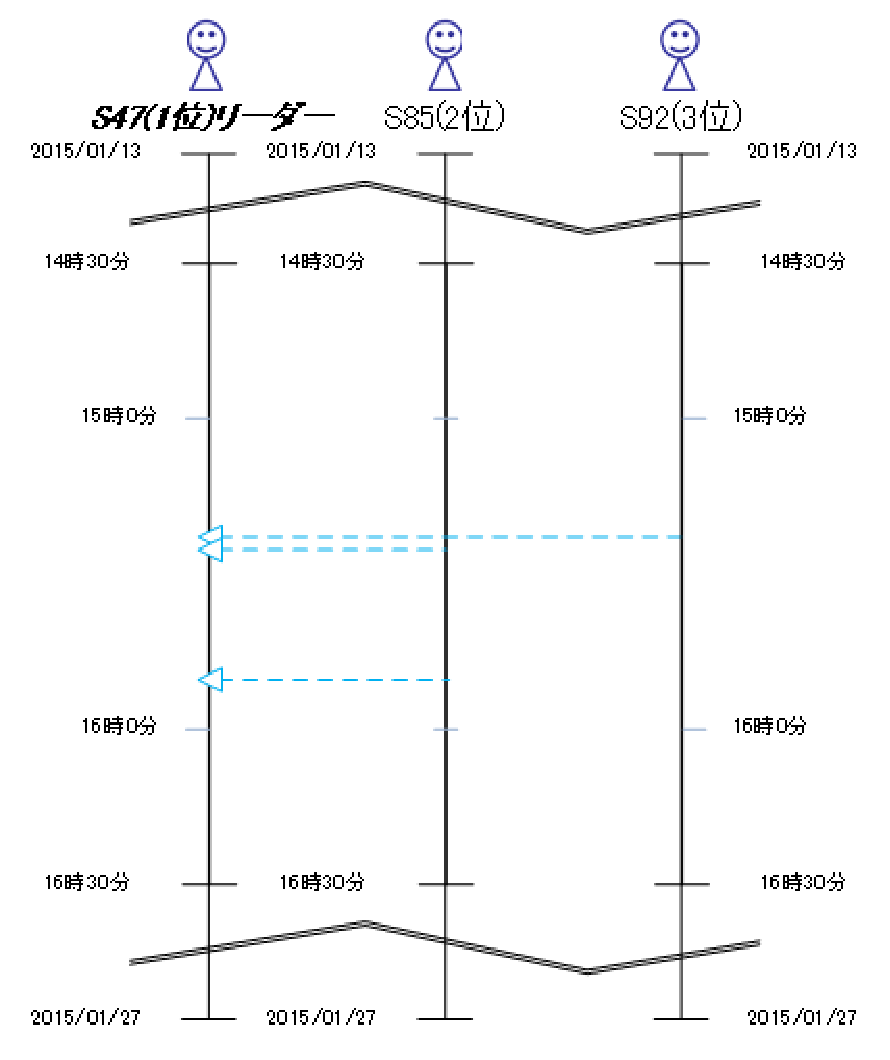
\includegraphics[scale=0.4]{img/flowK.eps}
		\caption{ソースコードの提供による貢献パターン(Group K)}
		\label{fig:flowK}
	\end{center}
\end{figure}

\begin{figure}[tb]
	\begin{center}
		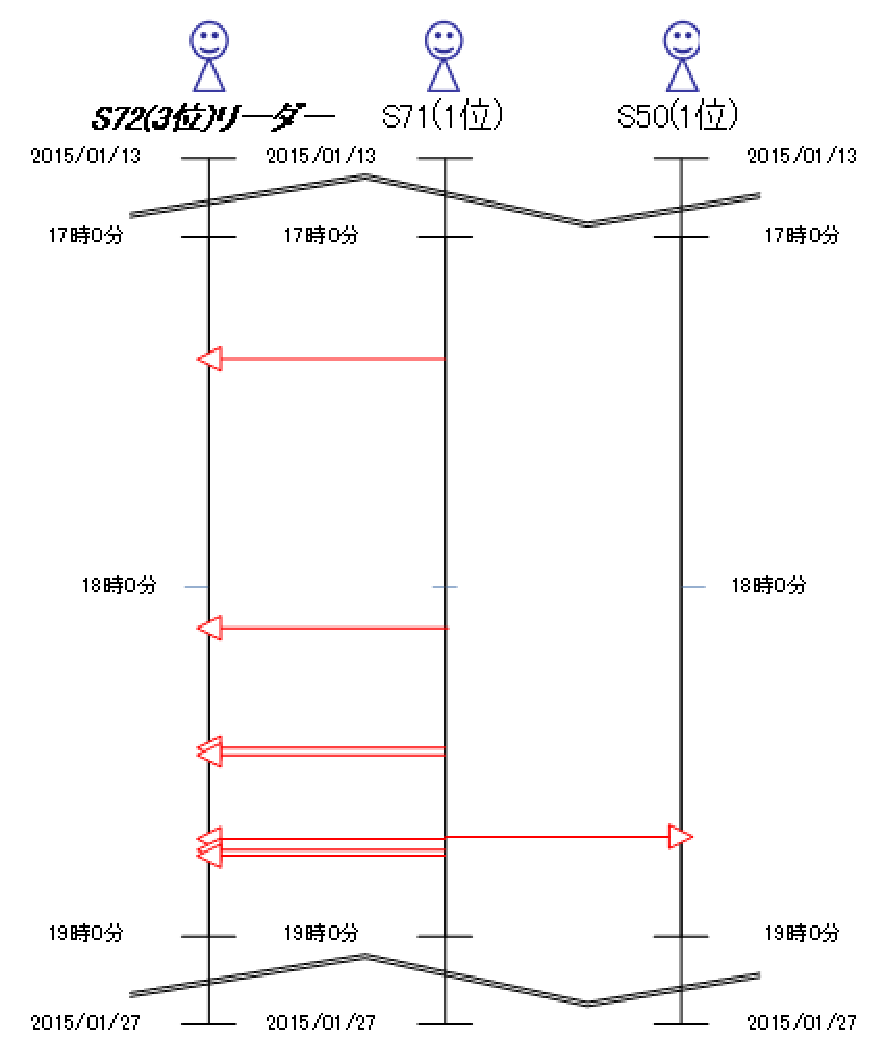
\includegraphics[scale=0.4]{img/flowL.eps}
		\caption{テストによる貢献パターン(Group L)}
		\label{fig:flowL}
	\end{center}
\end{figure}

\begin{figure}[tb]
	\begin{center}
		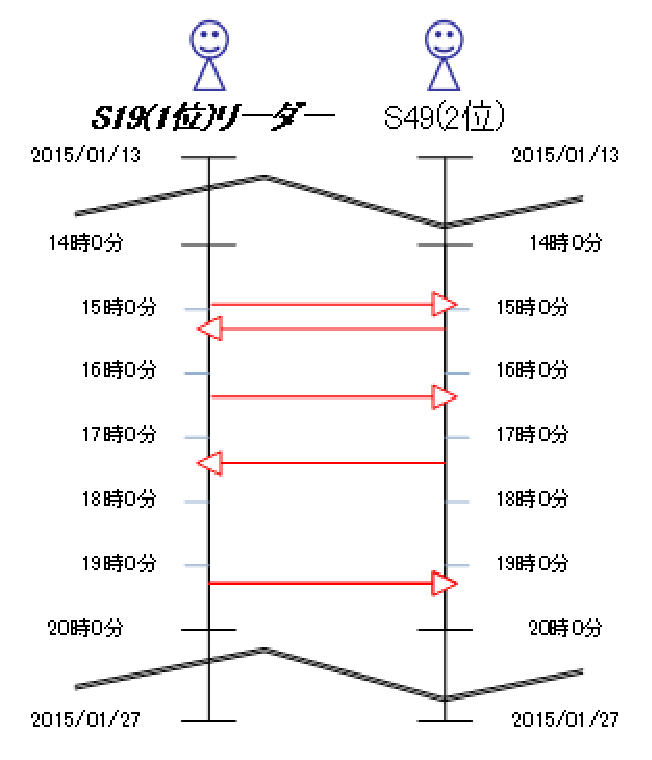
\includegraphics[scale=0.5]{img/flowE.eps}
		\caption{交互拡張(Group E)}
		\label{fig:flowE}
	\end{center}
\end{figure}

%----------7.2.1------
\subsection{ソースコードの提供による貢献}

フォロワが実装したプログラムの一部がドライバに取り込まれ,最終成果物の一部として採用されることがある.このパターンは全15グループ中7グループで見られた.

例としてグループKのインタラクション図の一部を\figref{fig:flowK}に示す.グループKのフォロワ(S85とS92)がドライバ(S47)のプロジェクトを全部取込していた.その後ドライバが各フォロワからプログラムの一部を取り込んでいる.

部分取込によって取り込まれたソースコードは,授業の教室を選ぶという,アドベンチャーゲームの1シーンである.S47はS85から別のシーンに関するソースコードも部分取込している.以上から,グループKのフォロワはそれぞれ担当するシーンについて責任を担い,実装をしていたと考えられる.


%----------7.2.2------
\subsection{テストによる貢献}

締め切り日の前夜にフォロワがドライバのプロジェクトを繰り返し全部取込するという現象が見られる.このパターンは全15グループ中6グループで見られた.

例としてグループLのインタラクション図の一部を\figref{fig:flowL}に示す.S72がS71から繰り返し全部取込をしていることから,フォロワがドライバのプログラムを繰り返しテストをするテスタとして貢献していると考えられる.ドライバのプログラムを何度も取り込んでいることから,テスト結果をドライバに報告し,ドライバがそれを基に修正をし,再びフォロワが全部取込を行ってテストをするというプロセスを繰り返している.

取り込み操作が容易なことから,変更が加わるたびに何度もテストを行うことに関して煩わしさが減少し,テストという観点でフォロワがプロジェクトに貢献しやすくなったと考えられる.


%----------7.2.3--------
\subsection{交互拡張}\label{Alternate extension}

グループメンバ同士で交互に全部取込をしている様子が見られる.このパターンは全15グループ中6グループで見られ,その全てが2人グループであった.

例としてグループEのインタラクション図の一部を\figref{fig:flowE}に示す.このパターンからは,ドライバとフォロワに関係なくお互いがプログラムを拡張していることが考えられる.グループEは,まずS49がS19の最新のものを取り込んでいる.取り込んだものを拡張して,拡張したものをS19が再度取り込んで拡張するということを繰り返してプロジェクトが進んでいると想定できる.


%----------7.3--------
\section{成績とインタラクション}


\begin{table}[tb]
	\caption{各グループメンバの成績} 
	\label{tab:records}
	\begin{tabular}{cc}
	\begin{minipage}{0.5\hsize}
  		\begin{center}
			\subcaption{グループL}\label{tab:groupL}
			\hbox to\hsize{\hfil
			\begin{tabular}{cc}\hline\hline
				ID		& 成績 \\\hline
				S72		& 51.5 \\
				S71		& 58.5 \\
				S50		& 58.5 \\\hline
			\end{tabular}\hfil}
		\end{center}
	\end{minipage}

	\begin{minipage}{0.5\hsize}
  		\begin{center}
			\subcaption{グループN}\label{tab:groupN}
			\hbox to\hsize{\hfil
			\begin{tabular}{cc}\hline\hline
				ID		& 成績 \\\hline
				S18		& 43.5 \\
				S30		& 54 \\
				S31		& 42.5 \\\hline
			\end{tabular}\hfil}
		\end{center}
	\end{minipage}
	\end{tabular}
\end{table}


\begin{figure}[tb]
	\begin{center}
		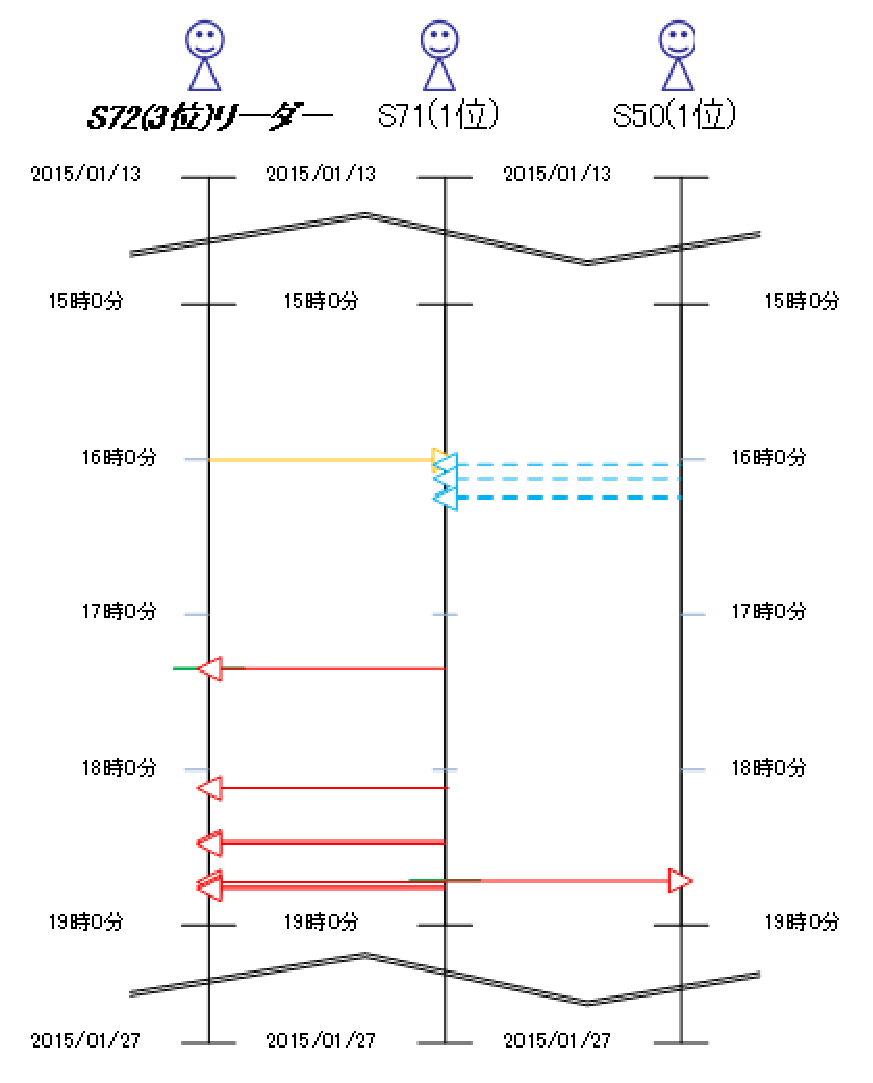
\includegraphics[scale=0.4]{img/flowL2.eps}
		\caption{グループLのインタラクション図}
		\label{fig:flowL2}
	\end{center}
\end{figure}


\begin{figure}[tb]
	\begin{center}
		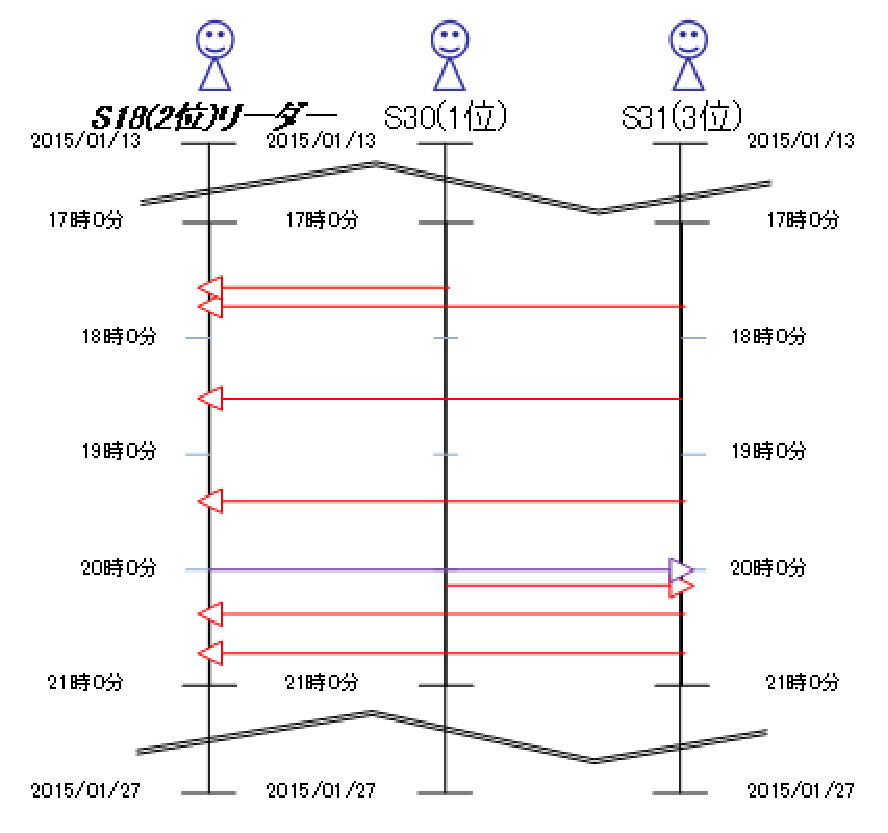
\includegraphics[scale=0.4]{img/flowN.eps}
		\caption{グループNのインタラクション図}
		\label{fig:flowN}
	\end{center}
\end{figure}


グループLのインタラクション図の一部を\figref{fig:flowL2},グループLの各メンバの成績を\tabref{tab:records}(a)に示す.S71は成績1位でドライバである.S50はドライバのS71ど同じ成績であり,ソースコードの一部で貢献している.S72は他のメンバと比べて成績が低く,テストで貢献している.

グループNのインタラクション図の一部を\figref{fig:flowN},グループNの各メンバの成績を\tabref{tab:records}(b)に示す.S30は成績トップでドライバである.S18はドライバのS30に比べて成績は低く,テストで貢献している.S31はS18と同等の成績でテストで貢献している.

以上のようなインタラクションから,各メンバが成績に見合った貢献ができていることがわかる.

\ref{Alternate extension}項で述べたように,交互拡張のパターンでは,各メンバが相手のソースコードを読んで拡張していることがわかる.しかし,グループN(\figref{fig:flowN})のように,成績差が大きいグループではソースコードの拡張までは行っていないメンバがいることがわかる.